\documentclass{beamer}
\usetheme{Boadilla}
\usepackage{essay-def}
\usepackage{bm}
\usepackage{amsfonts}
\usepackage{amssymb}
\usepackage{amsmath}
\usepackage{amsthm}
\usepackage{comment}
\usepackage{subcaption}
\usepackage{geometry}
\newcommand{\JX}[1]{{\color{red}{$^{\text{JX}}$[#1]}}}
\geometry{left=1cm,right=1cm}
    \title[Model Reduction]{Model reduction: past and present}
\author[ZJX]{Jiaxi Zhao}
\date{4th Dec, 2023}
\begin{document}
\par \setlength{\parindent}{2em}

\begin{frame}
\titlepage

\end{frame}

\begin{frame}{Words at the beginning}
	We will focus on \textbf{scientific} time series modeling. Model reduction is related to lots of other terminologies such as 
	modal analysis, reduced-order modeling, etc.

	The key feature of time series modeling:
	\begin{itemize}
		\item * Stability issue
		\item * Extrapolation or interpolation?
	\end{itemize}
	\begin{equation}
		\begin{aligned}
			& \mfX_1 \rightarrow \mfX_2 \rightarrow \cdots \mfX_n,		\\
			& t_1 \rightarrow \mfX_{t_1}, t_2 \rightarrow \mfX_{t_2}, \cdots
		\end{aligned}
	\end{equation}
\end{frame}

\begin{frame}{Reduced-order modeling: Past}
	\begin{itemize}
		\item Balanced Proper Orthogonal Decomposition (POD)
		\item Galerkin projection
		\item Discrete empirical interpolation method (DEIM)
		\item Koopman operator inspired methods
		\item Tensor-based methods\footnotemark
	\end{itemize}
	\footnotetext{Benner, Peter, et al., eds. Model reduction and approximation: theory and algorithms. Society for Industrial and Applied Mathematics, 2017.}
\end{frame}

\begin{frame}{Modal analysis: POD}
		\begin{figure}[ht]
			\centering
			\centerline{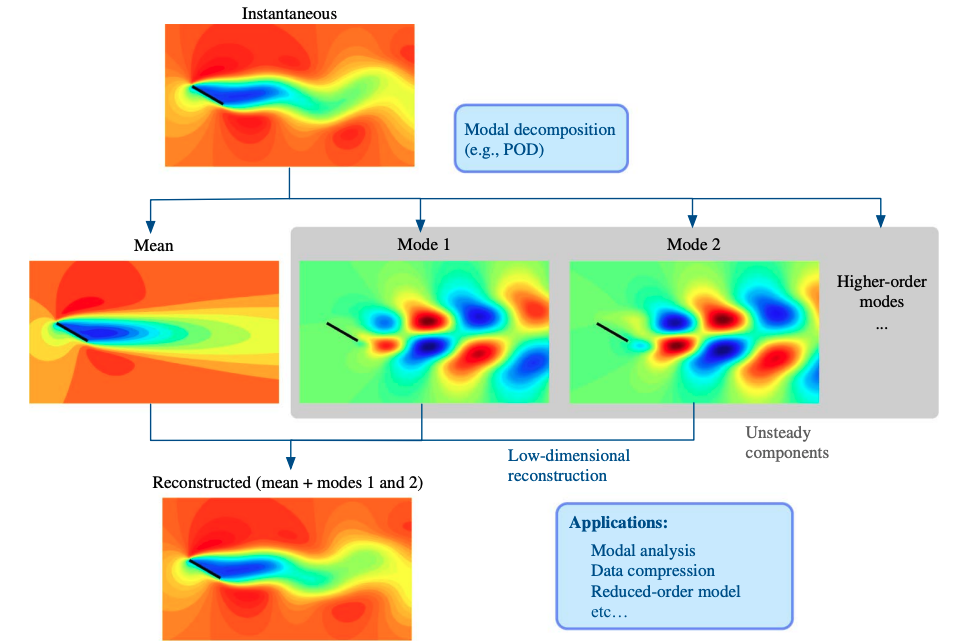
\includegraphics[width=.8\linewidth]{fig/POD.png}}
			\caption{Modal decomposition of two-dimensional incompressible flow over a flat-plate wing $Re=100, \alpha=30$. This example shows
			complex nonlinear separated flow being well represented by only two POD modes and the mean flowfield. Visualized are the streamwise velocity profiles.\footnotemark}
	\end{figure}
	\JX{What do these POD mean physically?}
		\footnotetext{Taira, Kunihiko, et al. "Modal analysis of fluid flows: An overview." Aiaa Journal 55.12 (2017): 4013-4041.}
\end{frame}

\begin{frame}{Balanced Transformation}
	Let us consider the following control system
	\begin{equation}
		\frac{d}{dt}\mfx(t) = A\mfx(t) + B\mfu(t), \quad \mfy(t) = C\mfx(t).
	\end{equation}
	The key observation is that any invertible transformation $\wtd \mfx = V\mfx$ will result in
	an equivalent system with different POD basis. For this system, the controllability and observability Grammians are defined as
	\begin{equation}
		W_c = \int_0^{\infty} e^{At}BB^T e^{A^Tt}dt, \quad W_o = \int_0^{\infty} e^{A^Tt}C^TC e^{At}dt.
	\end{equation}
	Balanced transformation $V$ is chosen so that the $W_c, W_o$ are diagonal and equal.
	\footnotemark
	\footnotetext{Willcox, Karen, and Jaime Peraire. "Balanced model reduction via the proper orthogonal decomposition." AIAA journal 40.11 (2002): 2323-2330.}
\end{frame}

\begin{frame}{Balanced POD}
	Under the transformation $V$, two Grammians will transform according to
	\begin{equation}
		\wtd W_c = V^{-1}W_cV^{-T}, \quad \wtd W_o = V^{T}W_oV.
	\end{equation}
	Then their product transforms as 
	\begin{equation}
		\wtd W_cW_o = V^{-1}W_cW_oV.
	\end{equation}
\end{frame}

\begin{frame}{Projection-based ROM}
	We consider two types of problem as follows:
	\begin{equation}
		\begin{aligned}
			\frac{d}{dt}\mfx(t) & = A\mfx(t) + N(\mfx(t)),\\
			0 & = A_{\mu}\mfx(\mu) + N_{\mu}(\mfx(\mu)), \quad \mfx \in \mbR^{n\times n}.
		\end{aligned}
	\end{equation}
	In both systems, $N(\cdot)$ represents the nonlinearity. Given any reduced basis functions of order $k$, 
	orthogonal projection operator onto this basis is denoted as $V_k$ with reduced system
	\begin{equation}
		\begin{aligned}
			\frac{d}{dt}\wtd\mfx(t) & = V_k^T A V_k\wtd\mfx(t) + V_k^T N(V_k\wtd\mfx(t)),\\
			0 & = V_k^T A_{\mu} V_k\wtd\mfx(\mu) + V_k^T N_{\mu}(V_k\wtd\mfx(\mu)), \quad \wtd\mfx \in \mbR^{k\times n}.
		\end{aligned}
	\end{equation}
\end{frame}

\begin{frame}{DEIM}
	The nonlinear term still remains huge amount of computation:
	\begin{equation}
		V_k^T N(V_k\wtd\mfx(t)), \quad \wtd J_N(\mfx(\mu)) = V_k^T J_F(V_k\wtd\mfx(\mu))V_k.
	\end{equation}
	The idea is to project this nonlinear term further onto a low-dimensional subspace spanned by $\lbb \mfu_0, \mfu_1, \cdots, \mfu_m \rbb$
	which is obtained by applying POD to the nonlinear snapshots obtained from the original full-order system.
	\begin{equation}
		N(V_k\wtd\mfx(t)) = \mfU c(t).
	\end{equation}
\end{frame}

\begin{frame}{Interpolation method}
	\footnotemark
	\footnotetext{Amsallem, David, and Charbel Farhat. "Interpolation method for adapting reduced-order models and application to aeroelasticity." AIAA journal 46.7 (2008): 1803-1813.
	}
\end{frame}

\begin{frame}{Difficulties of model reduction}
	\begin{itemize}
		\item * Nonlinearity, e.g. convection
		\item * Transient modeling and unsteady, especially for long time prediction and turbulence
	\end{itemize}
\end{frame}

\begin{frame}{Draw-back of linear-subspace ROM}
	In particular, linear-subspace ROMs can be expected to produce
	low-dimensional models with high accuracy\footnotemark only if the problem admits a fast decaying Kolmogorov n-width
	(e.g., diffusion-dominated problems). 
	\begin{equation}
		d_n(\mcM) := \inf_{\mcS_n}\sup_f\inf_{g\in\mcS_n}\|f-g\|.	
	\end{equation}
	Unfortunately, many problems of interest exhibit a slowly decaying
	Kolmogorov n-width (e.g., advection-dominated problems).
	\footnotetext{Binev, Peter, et al. "Convergence rates for greedy algorithms in reduced basis methods." SIAM journal on mathematical analysis 43.3 (2011): 1457-1472.}
\end{frame}

\begin{frame}{Koopman operator}
	Methods related to the Koopman operator are related to the dynamics of the operator,
	which is also approximated via a linear dynamics 
	\begin{itemize}
		\item * Extended Dynamical Model Decomposition (EDMD)
		\item * EDMD-DL 
		\item * parametric Koopman
	\end{itemize}
\end{frame}

\begin{frame}{ROM: Present}
	\begin{itemize}
		\item * Nonlinear ROM
		\item * Non-intrusive ROM via operator inference
		\item * Temporal coarsening
	\end{itemize}
\end{frame}

\begin{frame}{Nonlinear trial manifold: learn the reduced basis}
	Nonlinear trial manifold\footnotemark
	\begin{equation}
		\wtd \mfx(t;\mu)= \mfx_{ref}(\mu) + g(\wht \mfx(t;\mu)),
	\end{equation}
	where $\mfx_{ref}(\mu)$ denotes the parametrized reference state specified according to the initial condition and $g:\mbR^p \rightarrow \mbR^n$
	denotes the nonlinear parameterization function refered to as \textit{decoder}.	The reduced dynamics can be obtained via chain rule:
	\begin{equation}
		\frac{d}{dt}\wtd \mfx(t;\mu) = J_g(\wht \mfx(t;\mu))\frac{d}{dt}\wht \mfx(t;\mu).
	\end{equation}
	\footnotetext{Lee, Kookjin, and Kevin T. Carlberg. "Model reduction of dynamical systems on nonlinear manifolds using deep convolutional autoencoders." Journal of Computational Physics 404 (2020): 108973.}
\end{frame}

\begin{frame}{Time-continuous residual minimization}
	The model can be written using the residue function
	\begin{equation}
		\mfr(\mfv, \mfx, t, \mu) =  \mfv - f(\mfx, t, \mu).
	\end{equation}
	Based on this, we can define the equation for the reduced model as 
	\begin{equation}
		\frac{d}{dt}\wht \mfx(t;\mu) = \arg\min_{\mfv\in\mbR^p}\norml \mfr(J_g(\wht \mfx(t;\mu))\mfv, \mfx_{ref}(\mu) + g(\wht \mfx(t;\mu)), t, \mu) \normr
	\end{equation}
	Based on this, the truncation error analysis of the ROM can also be performed using approximation theory of the function spaces.
\end{frame}

\begin{frame}{Operator inference: Learn the reduced operator}
	
\end{frame}

\begin{frame}{Temporal coarsening}
	\begin{figure}[ht]
		\centering
		\centerline{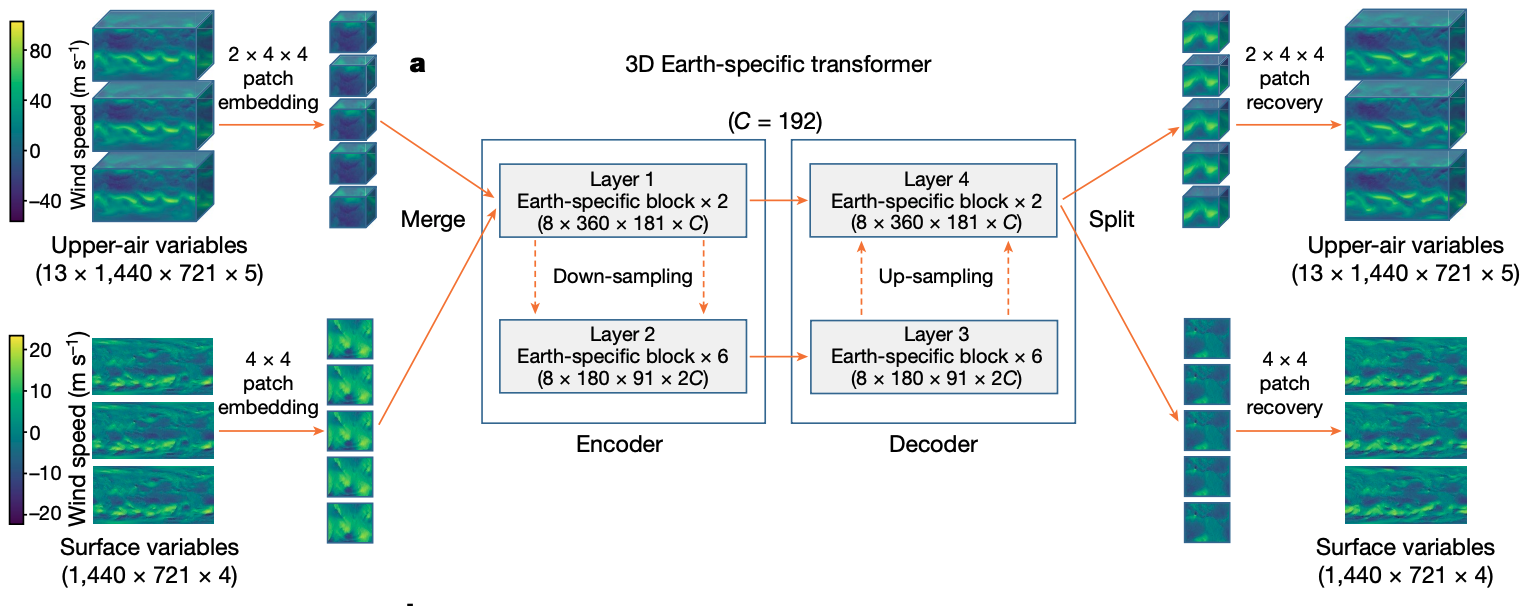
\includegraphics[width=\linewidth]{fig/pangu.png}}
		\caption{3DEST architecture.
		Based on the standard encoder–decoder design of vision transformers,
		we adjusted the shifted-window mechanism and applied an Earth-specific
		positional bias.\footnotemark}
\end{figure}
	\footnotetext{Bi, Kaifeng, et al. "Accurate medium-range global weather forecasting with 3D neural networks." Nature 619.7970 (2023): 533-538.}
\end{frame}

\begin{frame}{How to do long time prediction?}
	One of the bottleneck for ROM is the long time prediction accuracy: e.g. for weather forecasting,
	most data-driven models outperform numerical weather prediction over the 0-7 days regime but
	quickly 

	Several methods to perform time series prediction:
	\begin{itemize}
		\item * Hierarchical temporal aggregation
		\item * Manifold regularization
		\item * Nonlinear stability issue, especially compared with classical numerical stability
	\end{itemize}
\end{frame}

\begin{frame}{Operator inference ROM}
	Mesh-based $\Longrightarrow$ Mesh-free

	Another kind of nonlinear ROM is based on operator inference. A heuristic:
	Classical mesh-based solver amounts to solve the high dimesional mapping between the discretization on
	the huge mesh, e.g. $\mbR^{N\times N\times N} \rightarrow \mbR^{N\times N\times N}$, how about considering directly
	$\mbR^3 \rightarrow \mbR$, which is usually a nonlinear map\footnotemark.

	\textbf{Can be viewed as learning the reduced basis and operator simultaneously}
	\footnotetext{Mildenhall, Ben, et al. "Nerf: Representing scenes as neural radiance fields for view synthesis." Communications of the ACM 65.1 (2021): 99-106.
	}
\end{frame}

\begin{frame}{Operator inference ROM}
	More over, the parameter can also be fitted into this framework by encoding it as a latent vector\footnotemark
	\begin{figure}[ht]
		\centering
		\centerline{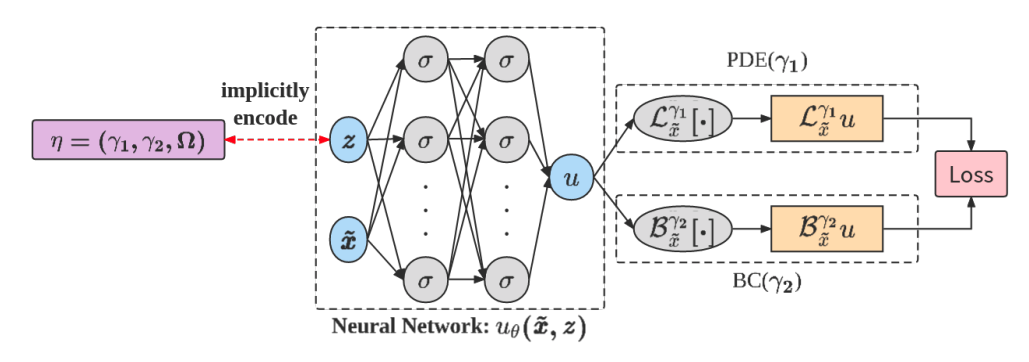
\includegraphics[width=\linewidth]{fig/MAD.png}}
		\caption{
		Architecture of Meta-Auto-Decoder..\footnotemark}
\end{figure}
	\footnotetext{Park, Jeong Joon, et al. "Deepsdf: Learning continuous signed distance functions for shape representation." Proceedings of the IEEE/CVF conference on computer vision and pattern recognition. 2019.
	}
\end{frame}

\begin{frame}{Relation to the sequence modeling}
	Given that present ROM are more and more similar to the sequence modeling in lots of CS application, i.e.
	non-intrusive method, similar transformer network. I personally think it worth to think carefully about their
	relationship.
	\begin{itemize}
		\item * Seq2Seq seems still not prevalent in scientific time series modeling.
		\item * Stability and out-of-distribution issue
	\end{itemize}
\end{frame}

\end{document}